\providecommand\ExamFontPath{../../../字体/}
\documentclass[fontset=exam]{exam-zh}
\usepackage{longtable,booktabs,array,calc,multirow,fvextra}
\usepackage[normalem]{ulem}
\providecommand{\hl}[1]{#1}
\providecommand{\ul}[1]{\uline{#1}}
\DefineVerbatimEnvironment{verbatim}{Verbatim}{breaklines=true,fontsize=\small}
\providecommand{\tightlist}{\setlength{\itemsep}{0pt}\setlength{\parskip}{0pt}}
\newcommand{\pandocbounded}[1]{#1}
\setlength{\emergencystretch}{3em}
\setlength{\tabcolsep}{2pt}
\examsetup{page/size=a4paper}
\title{厦门大学 2012 级期末试卷}
\subject[4em]{力学}
\begin{document}
\maketitle
\fancyfoot[C]{第 \thepage 页（共 \pageref*{LastPage} 页）}
\pdfbookmark[1]{一． 判断题（每小题2分，共20分。正确的在相应序号后打“√”，错误的打“×”。要求将答案写在答题纸上）}{section1}

一． 判断题（每小题 2 分，共 20 分。正确的在相应序号后打``√''，错误的打``×''。要求将答案写在答题纸上）

\begin{enumerate}
\def\labelenumi{\arabic{enumi}.}
\item
  当刚体作纯滚动时，作用在刚体上的静摩擦力总是与质心的运动方向相反。
\item
  刚体的质量越大，其转动惯量就越大，因而其转动惯性也越大。
\item
  作用在刚体上的外力的矢量和为零时，刚体的运动状态一定不变
\item
  驻波不是平面简谐波
\item
  一波源产生的平面简谐横波一段时间后将振动传播至某质点，该质点初始振动方向取决于它离波源的位置。
\item
  定常流动时的流线与流迹相重合
\item
  位移共振频率与振动系统的固有频率一般情况下总是完全相同。
\item
  在所有的惯性系中，真空光速具有相同量值，与光源的运动无关
\item
  列车进站时，站台上的乘客听到列车的汽笛声音调升高可用多谱勒效应解释。
\item
  动量和能量守恒定律在狭义相对论中仍然成立
\end{enumerate}

\pdfbookmark[1]{二．(16分)如图所示，质量为m_1，长为l的均匀细棒静止于水平桌面上。细棒可绕通过其端点O的竖直固定光滑轴转动。棒与桌}{section3}

二．(16 分)如图所示，质量为\(m_{1}\)，长为\(l\)的均匀细棒静止于水平桌面上。细棒可绕通过其端点 O 的竖直固定光滑轴转动。棒与桌面间的滑动摩擦因数为\(\mu\)。今有一质量为\(m_{2}\)的滑块在水平面内以垂直于棒长方向的速度\(v_{1}\)与棒的下端相碰，碰撞后滑块的速度变为\(v_{\text{2}}\)，方向与\(v_{1}\)相反。试求：\par\medskip{\centering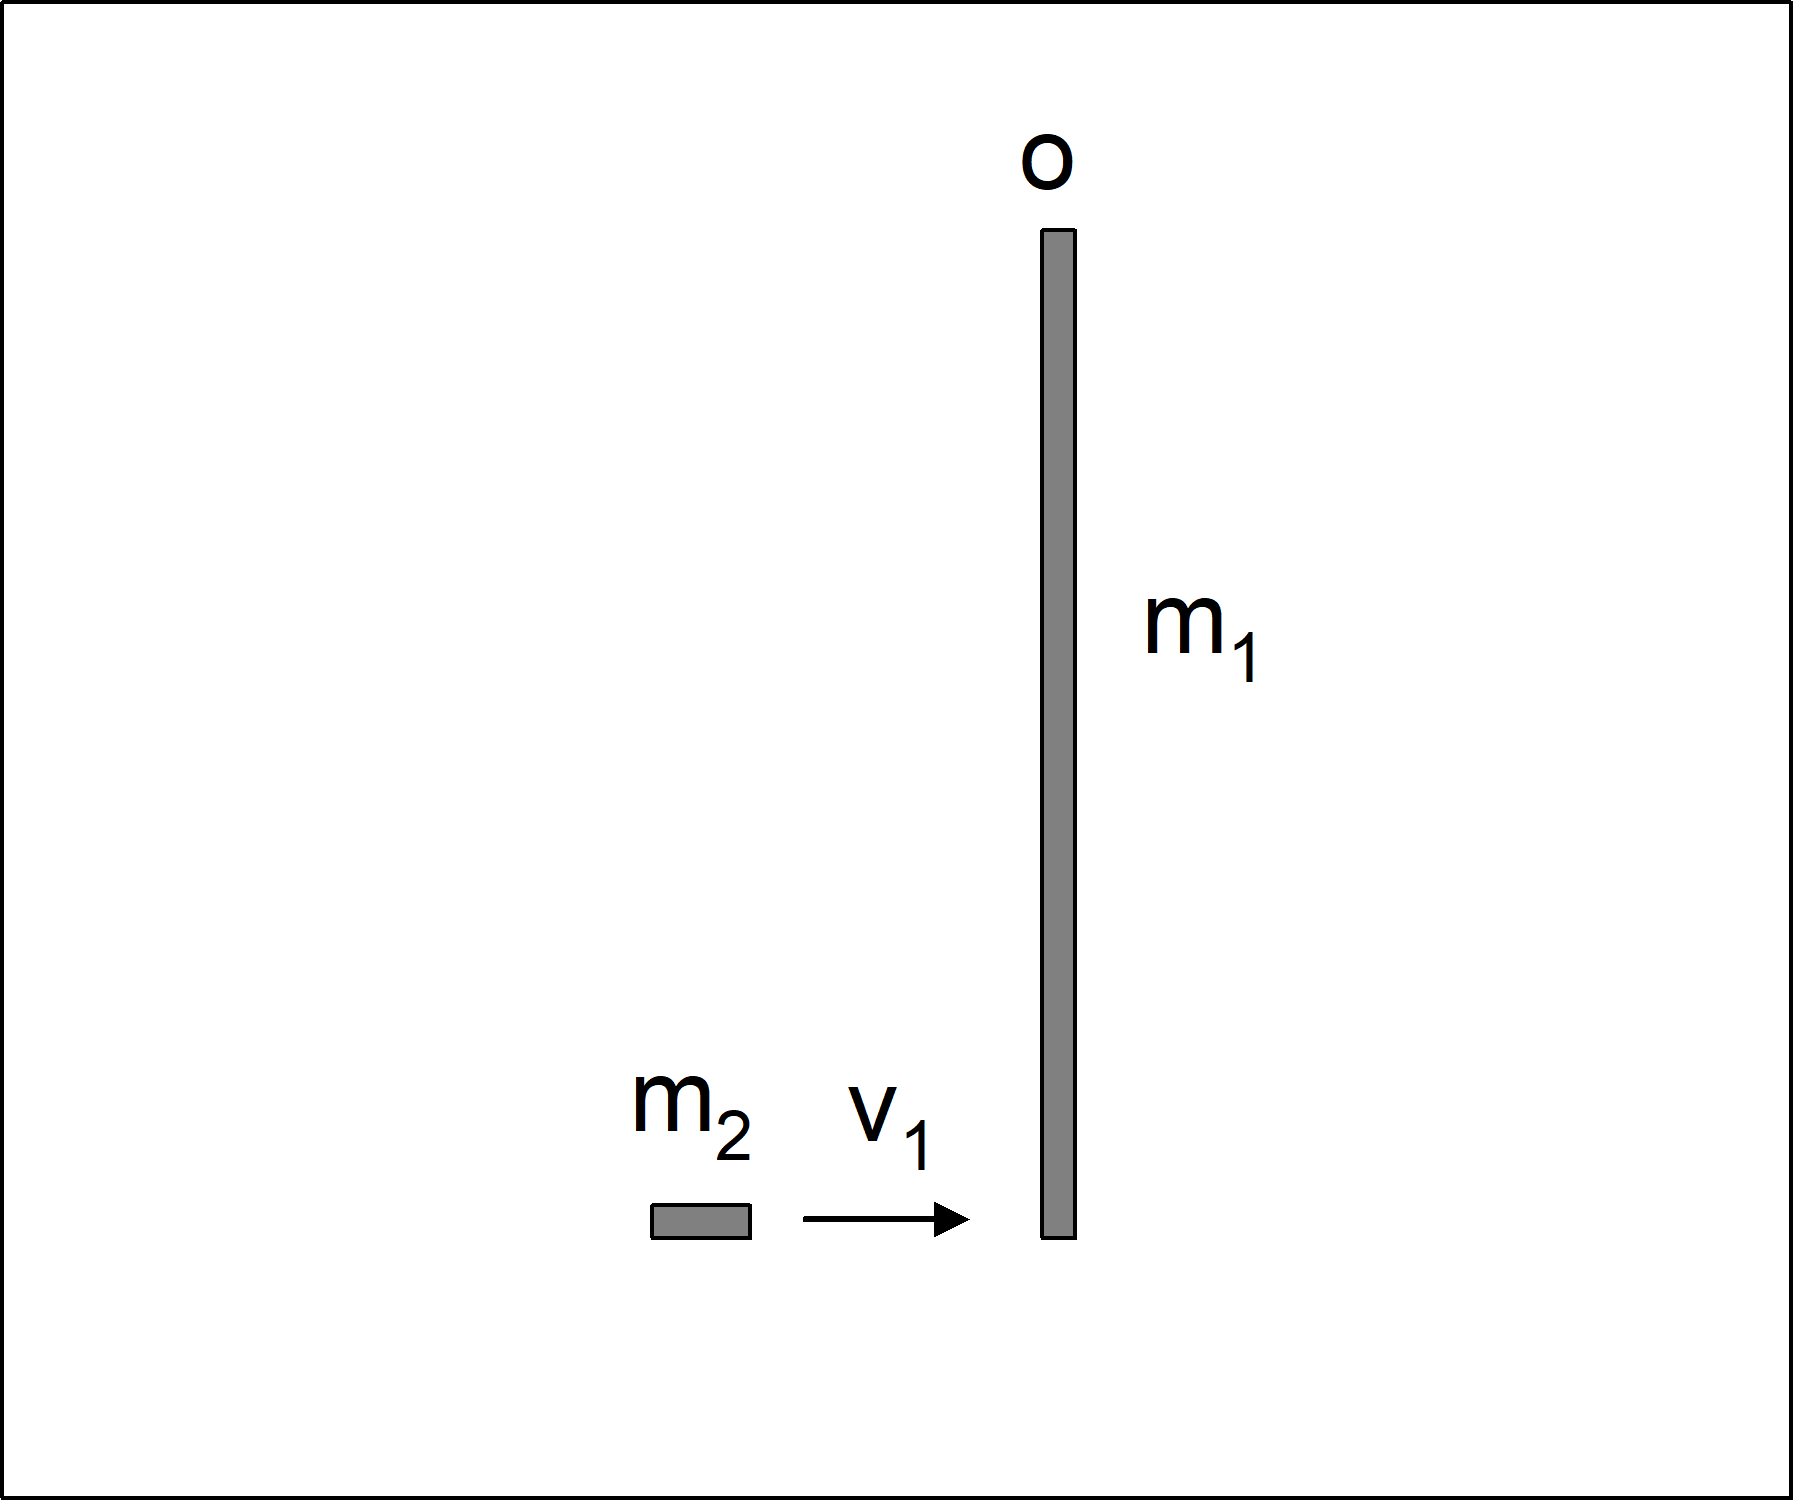
\includegraphics[width=5cm,height=4cm,keepaspectratio]{figures/image2.png}\par}\medskip

（1）滑块碰撞后棒所获得的角速度;

(2) 碰撞后棒在转动过程中所受的摩擦力矩;

(3) 碰撞后，从细棒开始转动到转动停止所经历的时间。

\pdfbookmark[1]{三．(16分)如图所示，质量为m的平板受水平力F的作用沿水平地面运动。板与地面的摩擦因数为mu。板上放一质量为M, 半径}{section7}

三．(16 分)如图所示，质量为 m 的平板受水平力 F 的作用沿水平地面运动。板与地面的摩擦因数为\(\mu\)。板上放一质量为 M, 半径为 R 的匀质圆柱体，圆柱体与板间的摩擦因数也为\(\mu\)。若圆柱体在板上的运动是纯滚动,求：

\par\medskip{\centering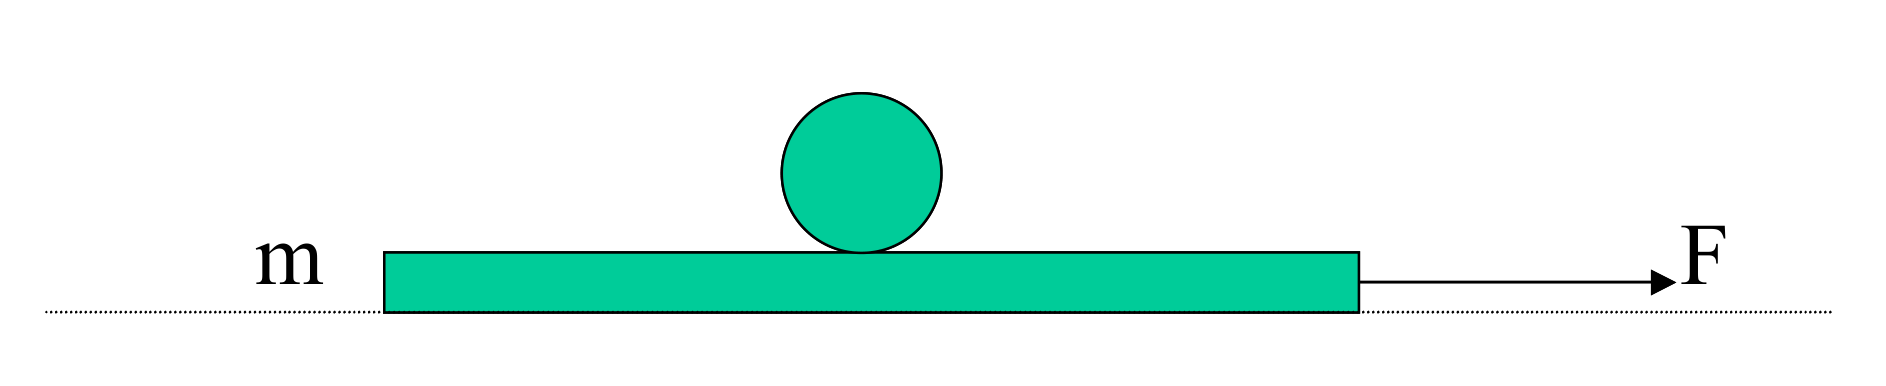
\includegraphics[width=5cm,height=4cm,keepaspectratio]{figures/plate3.png}\par}\medskip

　（1）板的加速度

　（2）圆柱体的角加速度。

\pdfbookmark[1]{四、(16分)如图所示，已知弹簧的劲度系数为k，物体的质量为m，滑轮的半径为R，质量为M。开始时托住物体m，使得系统保持}{section10}

四、(16 分)如图所示，已知弹簧的劲度系数为 k，物体的质量为 m，滑轮的半径为 R，质量为 M。开始时托住物体 m，使得系统保持静止，绳子刚好拉直而弹簧无形变，t=0 时放开 m。设绳子与滑轮间无相对滑动，滑轮可视为均质圆盘。\par\medskip{\centering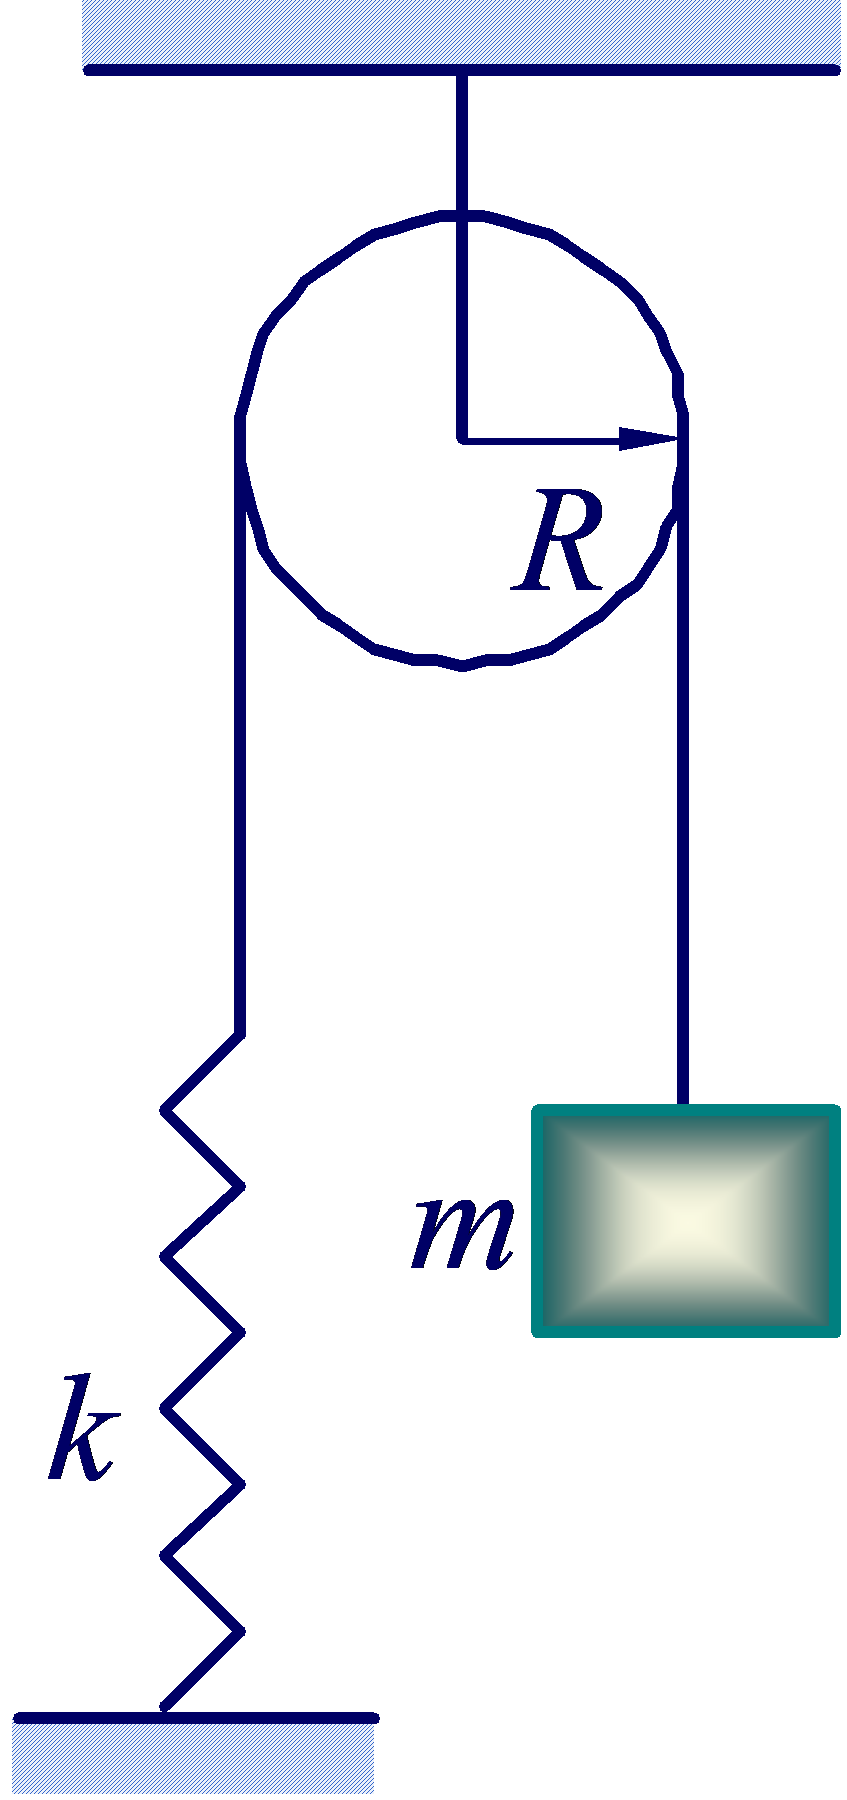
\includegraphics[width=5cm,height=4cm,keepaspectratio]{figures/image12.png}\par}\medskip

(1) 放开后 m 是否作简谐振动？若是，试求出振动周期 T；

(2) 写出 m 的振动表达式。

\pdfbookmark[1]{五．(16分)如图所示，一沿X轴正方向传播的平面简谐波从波疏媒质垂直入射到波密媒质上的B点并发生反射后形成的逆X轴传播的}{section13}

五．(16 分)如图所示，一沿 X 轴正方向传播的平面简谐波从波疏媒质垂直入射到波密媒质上的 B 点并发生反射后形成的逆 X 轴传播的反射波（振幅无衰减）。已知波源位于坐标原点 O 处，O 点到反射点 B 的距离 L=10 m，入射波的振幅\(A = 0.2\)(m)，频率\(\nu = 2\)(Hz)，波长λ=6m，当 t=0 时，波源离开平衡位置\(\sqrt{2}A/2\)，且向负 Y 方向运动，求:\par\medskip{\centering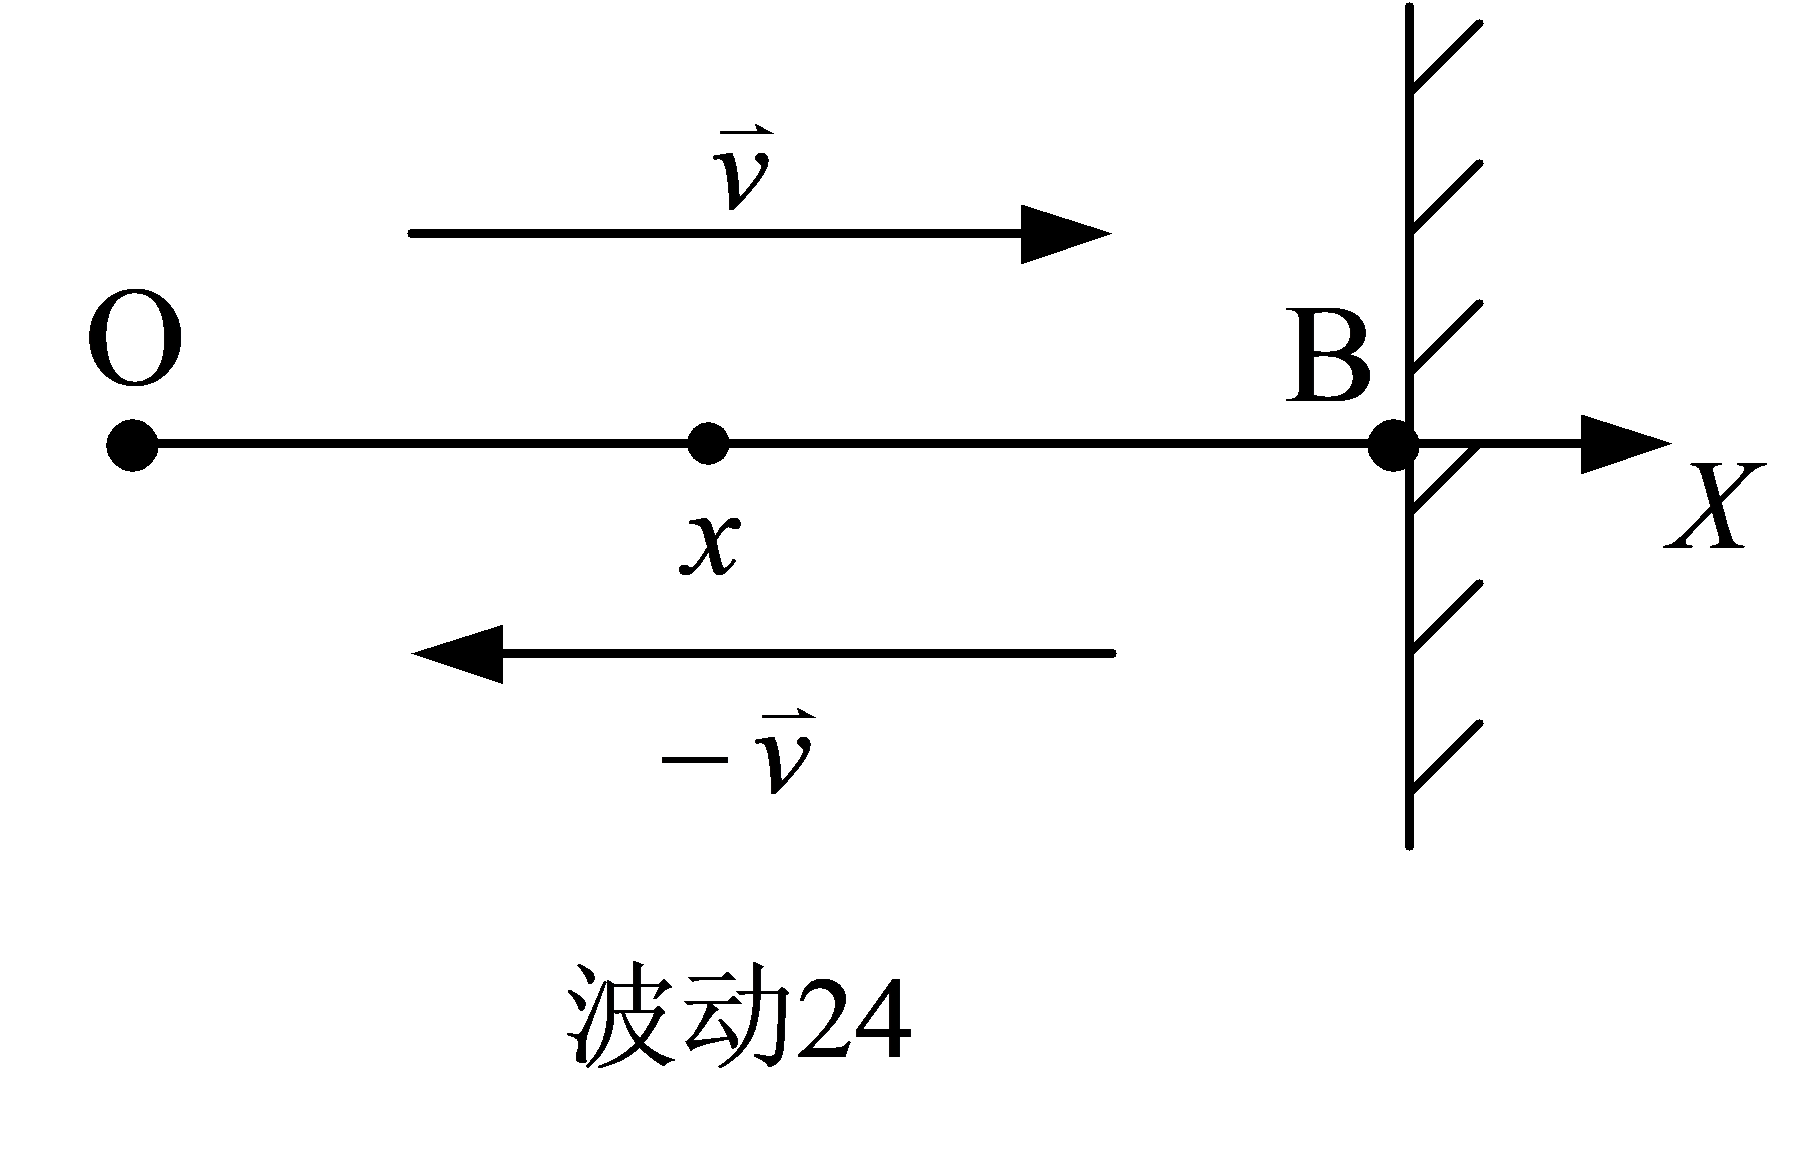
\includegraphics[width=5cm,height=4cm,keepaspectratio]{figures/image13.png}\par}\medskip

（1）入射波方程；

( 2 ) 反射波方程；

（3）OB 间因入射波和反射波干涉而静止的点的位置.

\pdfbookmark[1]{六. (16分)一宇宙飞船A相对地面以0.8c的速度于正午时刻飞经地球，此时飞船和地球上的观测者都把自己的时钟拨到12点}{section17}

六. (16 分)一宇宙飞船 A 相对地面以 0.8c 的速度于正午时刻飞经地球，此时飞船和地球上的观测者都把自己的时钟拨到 12 点。宇宙飞船上的宇航员测得飞船的长度为 50 米。问：

（1）地面上的观测者测得的飞船 A 的长度为多少？

（2）按飞船上的时钟，宇航员于午后 12 点 30 分飞经一星际宇航站。该宇航站相对地球固定，其站台时间指示的是地球时间。问飞船到达此宇航站时，站台时钟显示的时间是多少？

（3）若有另一飞船 B 相对地面以 0.8c 的速度沿相反方向飞行，问 A 飞船上的观测者所测得的 B 飞船的速度大小。

\end{document}
